\section{Interactions}

\subsection{Overview}

Here the system will be described in relations to names of commands and signals of the controller and other sensor components. Here is a picture that relates the names to the components.

\begin{figure}[!h]
	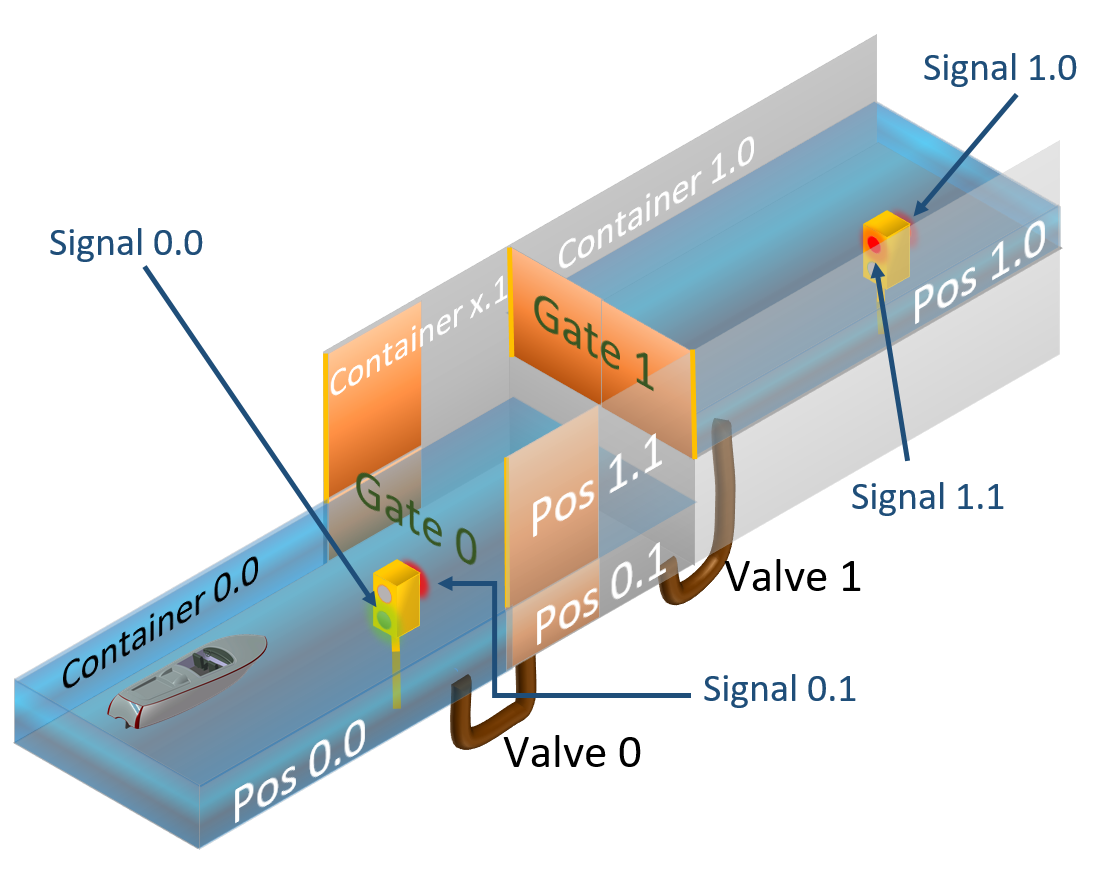
\includegraphics[width=\linewidth]{PictureName10}
	\caption{Description of the names}
	\label{fig:boat1}
\end{figure}
\pagebreak


\subsection{Commands}
\begin{table}[htbp]
	\centering
	\caption{Commands are given by the controller to the lift components and the ship operator/captain}
	\begin{tabular}{lll}
		\toprule
		\textbf{Actions} & \textbf{Description} & \textbf{Parameter} \\
		\midrule
		openGate & Open gate with the corresponding gate ID & gateID \\
		closeGate & Close gate with the corresponding gate ID & gateID \\
		openValve & Open valve with the corresponding gate ID & valveID \\
		closeValve & Close valve with the corresponding gate ID & valveID \\
		setSignalPass & Set signal to pass with the corresponding ID  & signalID \\
		setSignalHold & Set signal to hold with the corresponding ID  & signalID \\
		increaseWaterlevel & Container 1 water level increase & valveID \\
		decreaseWaterlevel & Container 1 water level decrease & valveID \\
		\bottomrule
		\end{tabular}%
		\label{tab:addlabel}%
		\end{table}%
		
		\pagebreak
		
		\subsection{Signals}
		\begin{table}[htbp]
			\centering
			\caption{These signals are generated in the lift components and sent to the controller per request (or the request is in the form of signals being sent constantly)}
			\begin{tabular}{lll}
				\toprule
				Actions & \textbf{Description} & \textbf{Parameter} \\
				\midrule
				requestGateState & Request gate state from gate.  & gateID \\
				receivedGateState & Returns open (true) or closed (false) & gateID \\
				\midrule
				requestValveState & Request valve state from gate. & valveID \\
				receivedValveState & Returns open (true) or closed (false) & valveID \\
				\midrule
				requestWaterflowState & Request waterflow state from valve. & valveID \\
				receivedWaterflowState & Returns on (true) or off (false) & valveID \\
				\midrule
				requestWaterlevel & Request waterlevel of two containters. & containerID \\
				receivedWaterlevel & Equal (true) or unequal (false) & containerID \\
				\midrule
				requestSignalState & Request the signal state from signal light & signalID \\
				receivedSignalState & Returns pass (true) or hold (false) & signalID \\
				\midrule
				requestGateSensor & Check if a ship is between the gate doors. & gateID \\
				receivedGateSensor & Returns if a ship is present (true) or not (false) & gateID \\
				\midrule
				requestShipPresence & Check a certain position if there is a ship present. & posID \\
				receivedShipPresence  & Returns if a sip is present (true) or not (false) & posID \\
				\bottomrule
				\end{tabular}%
				\label{tab:addlabel}%
				\end{table}%
				
				
